\usetikzlibrary{arrows.meta,calc}
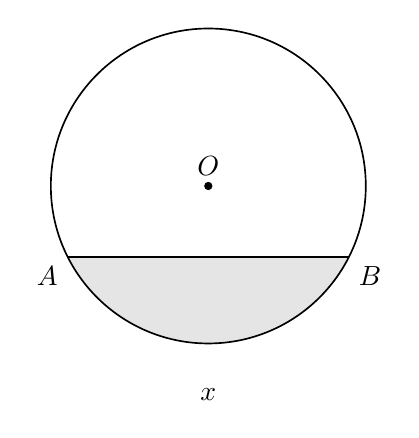
\begin{tikzpicture}[x=1cm,y=1cm,line width=.6pt,font=\normalsize,>=Stealth]
\coordinate (O) at (0,0);
\coordinate (A) at (-1.7857,-0.9);
\coordinate (B) at (1.7857,-0.9);
\fill[gray!20] (A) arc[start angle=206.76,end angle=333.24,radius=2.0cm] -- cycle;
\draw (O) circle[radius=2.0cm];
\draw (A)--(B);
\fill (O) circle (1.5pt);
\node[above] at (O) {$O$};
\node[below left] at (A) {$A$};
\node[below right] at (B) {$B$};
\node[below] at (0,-2.45) {$x$};
\end{tikzpicture}
